
%
% FDY TEMPLATE for Report
% ===================================================================
\NeedsTeXFormat{LaTeX2e}
\documentclass[11pt,twoside,a4paper]{fdyartcl}
\usepackage[utf8]{inputenc}
\usepackage[T1]{fontenc}
\usepackage[ngerman,english]{babel} % selectlanguage wird nur dann gebraucht, wenn
                                    % mehrere Sprachen-packages verwendet werden,
                                    % das zuletzt angegebene package ist die aktive
                                    % Sprache, mit \selectlanguage kann umgeschaltet
                                    % werden
\usepackage[intoc]{nomencl} % zur Erstellung einer Nomenklatur
                                   % Die Option [intoc] sorgt dafuer,
                                   % dass die Nomenklatur im
                                   % Inhaltsverzeichnis eingetragen
                                   % wird. Aufruf mit:
                                   % makeindex Diss.nlo -s nomencl.ist -o Diss.nls
\usepackage{longtable}  % fuer tabellen, die evtl ueber Seiten
                        % umgebrochen werden muessen
\usepackage{graphicx}   % Stellt \includegraphics zur Verfuegung
\usepackage{parskip}    % Setzt parindent auf null und parskip auf
                        % einen angemessenen Wert
\usepackage{calc}       % Erlaubt, verschiedene Masse zu addieren
                        % z.B 1cm+2pt
\usepackage[a4paper,twoside,outer=2.2cm,inner=3cm,top=1.5cm,bottom=2.7cm,includehead]{geometry}
                                        % erheblich verbesserte
                                        % Papieranassung
\usepackage{setspace}   % Stellt \singlespacing, \onehalfspacing und
                        % \doublespacig zur Verfuegung
                        % erlaubt ausserdem die Verwendung der
                        % Umgebung \begin{spacing}{2.3}
\setstretch{1.05}       % minimal vergroesserter Zeilenabstand
\usepackage{amsmath}    % Stellt verschiedene Mathematik Operatoren
                        % und Befehle bereit und verbessert die
                        % Darstellung von Gleichungen ermoeglicht
                        % ausserdem die Verwendung von \boldsymbol
                        % fuer z.B. griechische Buchstaben
\usepackage{amsfonts}
\usepackage{amsthm}
\usepackage{amssymb}
\usepackage{amsfonts}
\usepackage{harvard}    % neue citation Befehle und anderes Layout der
                        % Bibliographie
\usepackage{mathpazo}   % Aenderung der Standardschrift auf Palatino
\bibliographystyle{diss_harv_babel}
\input babelbst.tex     % sonst funktioniert das zweite \cite Kommando
                        % nicht, weil im harvardstyle \bbletal{}
                        % herausgeschrieben wird
%\usepackage{showkeys}   % Spaeter auskommentieren
\usepackage{upgreek}    % nicht-kursive grichische Buchstaben
\usepackage{fancyhdr}

\usepackage{ngerman}    %erlaubt auf allen Btriebssystemen die Eingabe der Umlaute als "a,"o,"u und "s mit dem Ergebnis
                        % ä,ö,ü und ß.(Gleiches gilt für Großbuchstaben)


%Packages for Compiling with PDFLatex using eps pictures
\usepackage{epstopdf}
\epstopdfsetup{update} % only regenerate pdf files when eps file is newer

\usepackage{enumitem} % Control layout of itemize, enumerate, description
\setdescription{
	labelindent=1em,
	leftmargin=.05\textwidth,
	style=nextline}


\graphicspath{{./Figures/}}%
% \input hyphen_dt.tex  % Spezielle Trennregeln fuer deutsche
                        % Woerter - gehoert in den Vorspann
\clubpenalty = 10000%
\widowpenalty = 10000%
\displaywidowpenalty =10000
% !TeX spellcheck = en_GB


%%%%%%%%%%%%%%%%%%%%%%%%%%%%%%%%%%%%%%%%%%%%%%%%%%%%%%%%%%%%%%%%%%%%%
%%%%%%%%%%%%%%%%%%%%%%%%%%%%%%%%%%%%%%%%%%%%%%%%%%%%%%%%%%%%%%%%%%%%%
% TITLE AND AUTHOR
%%%%%%%%%%%%%%%%%%%%%%%%%%%%%%%%%%%%%%%%%%%%%%%%%%%%%%%%%%%%%%%%%%%%%
%%%%%%%%%%%%%%%%%%%%%%%%%%%%%%%%%%%%%%%%%%%%%%%%%%%%%%%%%%%%%%%%%%%%%
\title{Tutorial}
\author{R. Mousavi B. T. - Chair of Fluid Dynamics - Darmstadt University of Technology}

%%%%%%%%%%%%%%%%%%%%%%%%%%%%%%%%%%%%%%%%%%%%%%%%%%%%%%%%%%%%%%%%%%%%%
%%%%%%%%%%%%%%%%%%%%%%%%%%%%%%%%%%%%%%%%%%%%%%%%%%%%%%%%%%%%%%%%%%%%%
%%%%%%%%%%%%%%%%%%%%%%%%%%%%%%%%%%%%%%%%%%%%%%%%%%%%%%%%%%%%%%%%%%%%%

%%%%%%%%%%%%%%%%%%%%%%%%%%%%%%%%%%%%%%%%%%%%%%%%%%%%%%%%%%%%%%%%%%%%%
%%%%%%%%%%%%%%%%%%%%%%%%%%%%%%%%%%%%%%%%%%%%%%%%%%%%%%%%%%%%%%%%%%%%%
% Kopfzeile
\pagestyle{fancy}
\fancyhf{}
\renewcommand{\headrulewidth}{0pt}

%\fancyhead[CE]{\sffamily \normalsize \thepage \quad \hrulefill \quad \sffamily \normalsize Short Title of Your Report }
%\fancyhead[CO]{\sffamily \normalsize F. Kummer \quad \hrulefill \quad \sffamily \normalsize \thepage }
\fancyhead[CE]{\sffamily \small \thepage \quad \hrulefill \quad \sffamily \small Tutorial }
\fancyhead[CO]{\sffamily \small BoSSS Documentation - April 15' \quad \hrulefill \quad \sffamily \small \thepage }


%%%%%%%%%%%%%%%%%%%%%%%%%%%%%%%%%%%%%%%%%%%%%%%%%%%%%%%%%%%%%%%%%%%%%
%%%%%%%%%%%%%%%%%%%%%%%%%%%%%%%%%%%%%%%%%%%%%%%%%%%%%%%%%%%%%%%%%%%%%

% Angaben fuer die Nomenklatur
%\makenomenclature
%\renewcommand{\nomname}{Nomenklatur}
%\setlength{\nomitemsep}{-0.2\parsep}% Der Abstand zweier Eintraege in
                                    % der Nomeklatur betraegt

% Dieser Befehl stellt sicher, dass neue Kapitel auf rechten (ungeraden) Seiten beginnen
\newcommand{\clearemptydoublepage}%
{\newpage{\pagestyle{empty}\cleardoublepage}}
\newfont{\myrm}{cmr12 at 12 pt}
% FigureXYLabel - urspruenglich in defin.tex, von Prof.~Dr.-Ing.~M. Oberlack
% Urspruengliche Version umfasste 5 Parameter -  geaenderte 7 Parameter - Bauerbach
% 1 Figurename: \includegraphics[......
% 2 Beschriftung der x Achse
% 3 x-Beschriftung - Verruecken horizontal positiv nach links
% 4 x Beschriftung - Verruecken vertikal positiv nach unten
% 5 Beschriftung der y Achse
% 6 y-Beschriftung - Verruecken horizontal positiv nach links
% 7 y Beschriftung - Verruecken vertikal positiv nach oben
\newlength{\FigureHeight}
\newlength{\FigureHeightHalf}
\newcommand{\FigureXYLabel}[7]{%
\settoheight{\FigureHeight}{#1}%
\setlength{\FigureHeightHalf}{0.5\FigureHeight}%
\addtolength{\FigureHeightHalf}{#7}%
\raisebox{\FigureHeightHalf}{\makebox[0cm][r]{#5\makebox[#6]{}}}%
#1\\%
\vspace{#4}%
{\makebox{#2\makebox[#3]{}}}}

%%%%%%%%%%%%%%%%%%%%%%%%%%%%%%%%%%%%%%%%%%%%%%%%%%%%%%%%%%%%%%%%%%%%%
%\addtokomafont{sectioning}{\rmfamily}
%\addtokomafont{section}{\normalsize}
%\addtokomafont{subsection}{\normalsize}

%\usepackage{sectsty}
%\sectionfont{ \parskip=0mm \vspace*{-5mm} }
%\subsectionfont{ \parskip=0pt \vspace*{-1mm} \centering \normalfont \normalsize \itshape}
%\paragraphfont{ \normalfont \itshape }

%       DOKUMENT
\begin{document}

\pagenumbering{arabic} % Zurueckschalten auf arabische Ziffern, dabei wird der Zaehler auf 1 gesetzt

%%%%%%%%%%%%%%%%%%%%%%%%%%%%%%%%%%%%%%%%%%%%%%%%%%%%%%%%%%%%%%%%%%%%%%%%%%%%%%%%55
% Seitennummer der ersten Seite
\setcounter{page}{1} % must be an odd number
                       % muss eine ungerade Zahl sein
%%%%%%%%%%%%%%%%%%%%%%%%%%%%%%%%%%%%%%%%%%%%%%%%%%%%%%%%%%%%%%%%%%%%%%%%%%%%%%%%55
%%%%%%%%%%%%%%%%%%%%%%%%%%%%%%%%%%%%%%%%%%%%%%%%%%%%%%%%%%%%%%%%%%%%%%%%%%%%%%%%55
%%%%%%%%%%%%%%%%%%%%%%%%%%%%%%%%%%%%%%%%%%%%%%%%%%%%%%%%%%%%%%%%%%%%%%%%%%%%%%%%55

% Titelseite
% -------------------
\maketitle

\begin{abstract}
The present document is a part the of the documentation written for the in-house computational code BoSSS, which can be used as a tutorial to start working with the code. The details of the numerical methods used in BoSSS are not considered in this document, rather the practical ways to use and develop BoSSS are discussed. The tutorial is started with a brief description on the layer structure of BoSSS. In the second section the database of BoSSS is briefly described. In the third section the installation procedure of BoSSS is described. The forth section is assigned to an introduction about the object-oriented programming in C\#, because BoSSS is written and has to be developed in this programming approach. The fifth section includes the examples which are started by solving a single two-dimensional scalar-transport equation. The next sub-sections are assigned to solving a set of two- and three-dimensional scalar-transport equations. The fifth section is continued by solving single- and multi-phase fluid problems governed by the Navier-Stokes equations, both in two and three dimensions. More examples will be added as more features are implemented in BoSSS.
\end{abstract}
%==================== Hauptteil =====================================
\section{A brief description on the architecture of BoSSS}
Working with BoSSS needs to know the architecture on which basis it is designed. In fact BoSSS is developed in five layers which are successively dependent to the lower layers. The libraries are named as L0 to L4. The first four layers contains various {\scriptsize .dll} files corresponding to the different libraries to be used for developing the applications in the fifth layer. In each layer containing libraries, one of the libraries is the primary library which is dependent on the libraries of the lower layers. The rest of the libraries are the auxiliary libraries which are dependent on the primary library of the corresponding layer and also the libraries of the lower layers. To name the {\scriptsize .dll} files, the dependencies are represented by {\scriptsize dot} sign. If the name of a {\scriptsize .dll} file contains the word {\scriptsize BoSSS} and another word with a {\scriptsize dot} sign between them, that file is a primary library like {\scriptsize BoSSS.Platform.dll}. The file {\scriptsize BoSSS.Platform.LinAlg.dll} is an auxiliary library which is dependent on the library {\scriptsize BoSSS.Platform.dll}. Each layer can be described briefly as the following:
\begin{itemize}
\item L0: This layer contains the libraries which are not programmed in BoSSS project. However these libraries are not programmed in C\#. The primary library of this layer is {\scriptsize Platform-Native.dll}.
\item L1: The libraries contained in this layer and the next layers are programmed in C\# in BoSSS project. The libraries which are included in layer 1, provides an interface between the C\# programmed part of the code and the non-C\# parts. The primary library of this layer is {\scriptsize BoSSS.Platform.dll}.
\item L2: This layer contains the libraries defining the fundamental concepts which are involved in BoSSS as a computational code applying the Discontinuous Galerkin method, such as grids, DG fields and operators. This layer also contains the input-output (IO) staffs. The primary library of this layer is {\scriptsize BoSSS. Foundation}.
\item L3: This layer contains the libraries related to the time discretization and some utilities. The primary library in this layer is {\scriptsize BoSSS.Solution}.
\item L4: This layer contains no library. Rather, the applications such as the solvers for scalar-transport equations or Navier-Stokes equation are developed in this layer. In other word, this layer is the work place for non-administrator developers and users. There are some applications already developed in this layer such as the incomplessible Navier-Stokes solver. But generally a user can start developing his/her own application in this layer from a VS (Visual-Studio) empty page.
\end{itemize}
\section{A brief description on the database of BoSSS}
Figure (1) represents the the database concept in BoSSS. The grid which is needed for a numerical calculation, is generated by a grid generation software. A tool which is called gridtool, is designed in the BoSSS project to convert the grid file to the special format which can be read by BoSSS. This tool imports the grid data to the BoSSS database. A BoSSS application can read the grid data from the BoSSS database. The solution data which is produced by a BoSSS application is saved in the BoSSS database. Using a tool which is called DBE (database explorer) and is designed in BoSSS project, the solution data is exported from the BoSSS database to a postprocessing software.
\begin{figure}[h] % htb: preferred position of picture: here, top, bottom of page
  \begin{centering}
  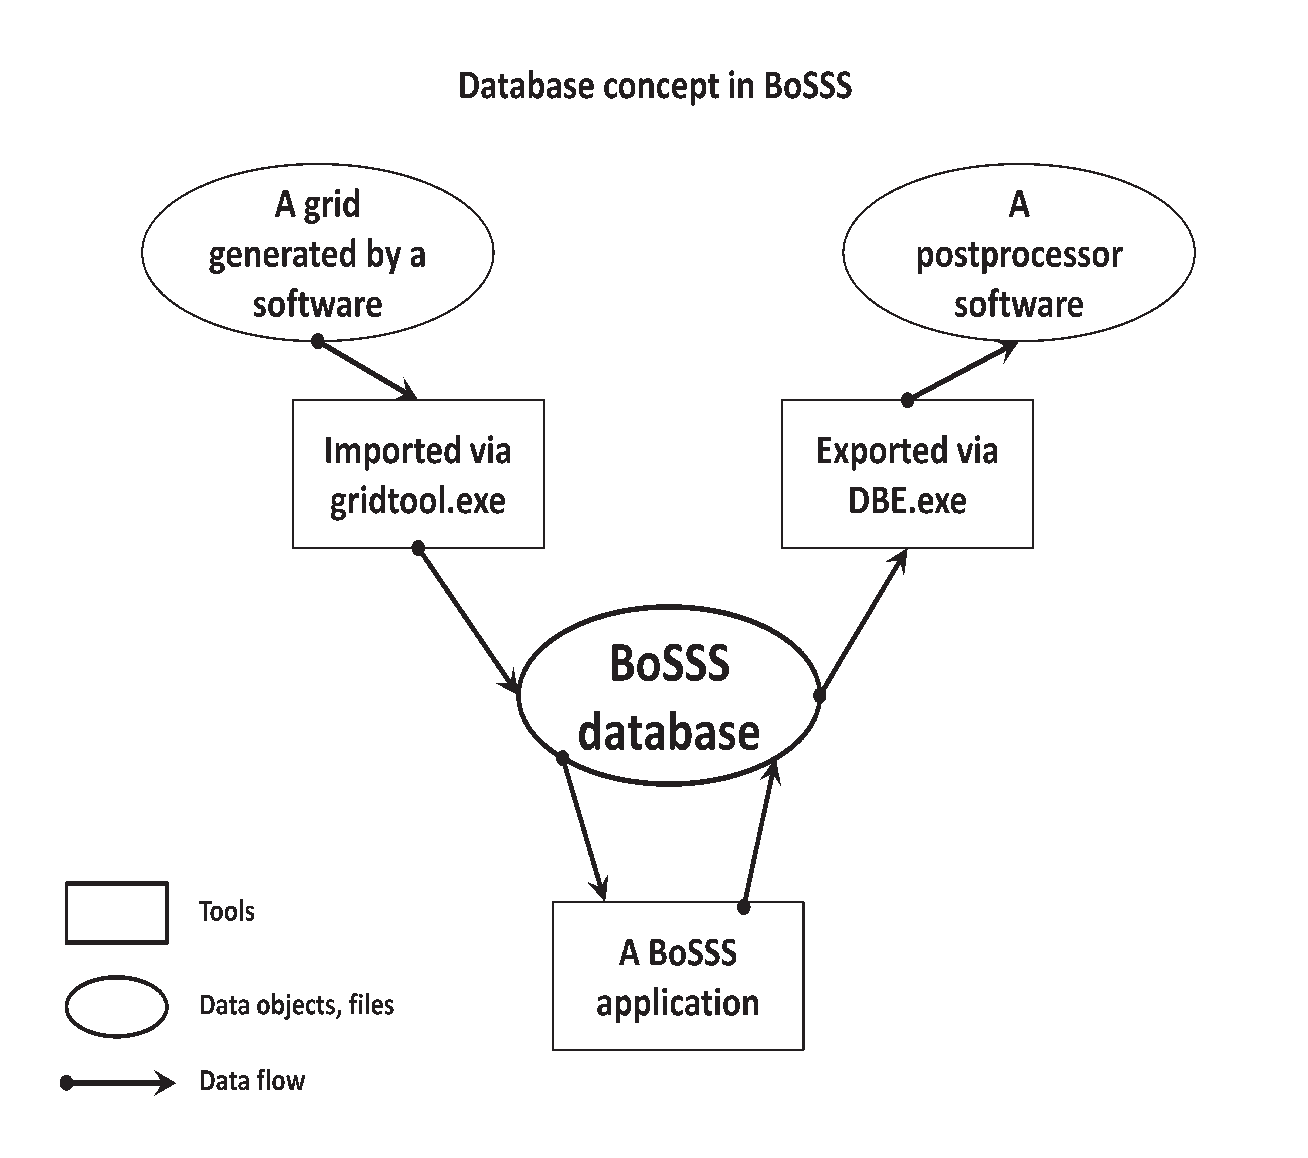
\includegraphics[width=0.5\textwidth]{Figures/DB}\\
  \end{centering}
  \caption{A flowchart representing the BoSSS database}
\end{figure}
\section{Installation of BoSSS on a PC located in fdy network}
\subsection{Introduction}
The installation of BoSSS is the procedure of copying a set of the files from a global repository to a local repository. The global repository ({\scriptsize \textbackslash\textbackslash fdyprime\textbackslash bosss\textbackslash root3}) is a place on the fdy file server for saving the original version of the code. The global repository can be mapped to a drive {\scriptsize R} in a PC in the fdy network by doing the following steps:
\begin{enumerate}
\item clicking {\scriptsize Start $\rightarrow$ Run}
\item executing the following command:
{\scriptsize \begin{verbatim}
  net use R: \\fdyprime\bosss/persistent:no
\end{verbatim}}
\end{enumerate}
The local repository is a place on a PC in the fdy network containing a copy of BoSSS. It is recommended to locate the local repository in the directory {\scriptsize C:\textbackslash BoSSS} or {\scriptsize C:\textbackslash Users\textbackslash user-name\textbackslash BoSSS}. There is also an exchange repository ({\scriptsize \textbackslash\textbackslash fdyprime\textbackslash bosss\textbackslash users\textbackslash user-name\textbackslash}) where is a place on the fdy file server where the developers and users can exchange their own developments. Every developer and user has his own directory on this place. There are two types of the files contained in the global repository, including the files which are tracked by the software Git after copying to the local repository, and the files which are not tracked by this software. The files contained in the directories which have the names with the suffix {\scriptsize .git} are tracked by Git. Git is a software to manage the source code development of a software in a team of developers. Pulling the updates from the global and exchange repositories to a local repository and pushing the new developments to the exchange repository, can be done using this software. The text version of Git is called Git-Bash. There is also a GUI version of the software which is called Git-Extension. The software can be freely downloaded from the internet. The files which are not tracked by Git can be copied normally. But the files which are tracked by Git must be copied using Git. Figure (2) shows a flowchart representing he global, exchange and local repositories.
\begin{figure}[h] % htb: preferred position of picture: here, top, bottom of page
  \begin{centering}
  \includegraphics[width=1\textwidth]{Figures/git}\\
  \end{centering}
  \caption{A flowchart representing the global, exchange and local repositories}
  \label{git-structure}
\end{figure}
\subsection{Directory structure of BoSSS}
 Prior to copying the files, the directory structure of BoSSS should be known. Both in the global and local repositories, the main directory has the sub-directories with the following structure:
\begin{itemize}
\item src: This directory contains the parts of BoSSS which are available for the developers and users. The sub-directories of this directory are as the following:
    \begin{itemize}
    \item public.git: This directory which is tracked by Git, contains the public available parts of BoSSS (see section (4.10)).
    \item DBE.git: This directory which is tracked by Git, contains the source code of BoSSS database explorer.
    \item Utils.git: This directory which is tracked by Git, contains some utilitie.
    \item protected: This directory contains the protected available parts of BoSSS (see section (4.10)).
    \item private: This directory contains the developer-specific parts of BoSSS which should not be available for the other developers or users at the moment.
    \item MySolution: This directory contains VS solution file(s) created by a developer or user. The name of this directory is arbitrary.
    \end{itemize}
\item etc: This directory contains almost all of the configuration files for tools like DBE (database explorer) or bcl (BoSSS command line) ...
\item bin: This directory contains all of the .dll files to be used in BoSSS. The following sub-directories belong to this directory:
    \begin{itemize}
    \item Debug: This directory contains the {\scriptsize .dll} files corresponding to the debug build of the C\# - coded parts of BoSSS.
    \item Release: This directory contains the {\scriptsize .dll} files corresponding to the release build of the C\# - coded parts of BoSSS.
    \item native: This directory contains the {\scriptsize .dll} files corresponding to the platform-dependent parts of BoSSS including the 3rd party codes like Hypre, MUMPS, ... which are developed in different programming languages. This directory contains a sub-directory as the following:
        \begin{itemize}
        \item win32: This directory contains the {\scriptsize .dll} files corresponding to the 32-bit version of the code.
        \end{itemize}
    \end{itemize}
\item doc: This directory contains the documentations of BoSSS. The following sub-directories belong to this directory:
    \begin{itemize}
    \item ref: This directory contains the reference manual of BoSSS. This reference manual which is created by the software Sandcastle, is the collection of the comments written in the different C\#-coded parts of BoSSS.
    \item notes.git: This directory which is tracked by Git, contains several documentations corresponding to the different topics involved in BoSSS.
    \end{itemize}
\item tmp: This directory is an auxiliary directory for temporary created files
\item plots: This directory is a place to save the plot files created by the tool DBE. This directory has the following sub-directories:
    \begin{itemize}
    \item projects: This directory contains the plot files created in different particular projects in the tool DBE.
    \item sessions: This directory contains the plot files created in different sessions in the tool DBE.
    \end{itemize}
\end{itemize}
\subsection{Automatic installation}
There is an installer designed to automatically copy the files from the global repository to the local repository: %, using Git, as the following steps:
%\begin{enumerate}
%\item Make an arbitrary directory in your PC, let's say {\scriptsize C:\textbackslash BoSSS}, as the local repository.
From the directory {\scriptsize R:\textbackslash bosss\textbackslash install \textbackslash }, run the newest installation file {\scriptsize BoSSS-inst-XXX.exe}.\\
% to somewhere in your PC, let's say for example {\scriptsize C:\textbackslash temp}.
%\item In Git-Bash, execute the following command to be inside the directory where you have located the file {\scriptsize BoSSS-ins.exe}:
%    {\scriptsize \begin{verbatim}
%    cd /c/temp (recommended: C/Users/username/AppData/Local/BoSSS)
%    \end{verbatim}}
%\item In Git-Bash, execute the following command to get some instructions:
%    {\scriptsize \begin{verbatim}
%    BoSSS-inst.exe
%    \end{verbatim}}
%\item In Git-Bash, execute the following command to copy the files from the global repository to the local repository:
%    {\scriptsize \begin{verbatim}
%    BoSSS-inst --isrc /r/root --root /c/BoSSS
%    \end{verbatim}}
%\end{enumerate}
%After these steps, the mentioned sub-directories in the section (3.2) are created in the directory {\scriptsize C:\textbackslash BoSSS}.\\
%To be able to use BCL, the following steps should be done:
%\begin{enumerate}
%\item In Git-Bash execute the following command to be inside the directory {\scriptsize C:\textbackslash BoSSS} where the file {\scriptsize setvars.sh} is located:
%{\scriptsize \begin{verbatim}
%  cd /c/BoSSS
%\end{verbatim}}
%\item In Git-Bash execute the following command:
%{\scriptsize \begin{verbatim}
%  ./setvars.sh
%\end{verbatim}}
%\end{enumerate}
%After doing these steps, a description about BCL can be shown by executing the following command:
%{\scriptsize \begin{verbatim}
%  bcl.exe
%\end{verbatim}}
The next step is initiating a data-base for saving the data files created after running the BoSSS applications. \\
\emph{Remark:} For this step a valid control file for the Database Explorer {\scriptsize DBY.xml} must be placed in the users config folder. Currently one has to refer to an administrator to get such a file.\\
It is recommended to initiate the database on an fdy network derive. To do that, the following steps should be done:
\begin{enumerate}
\item In Git-Bash execute the following command to be inside the directory {\scriptsize P:\textbackslash}:
    {\scriptsize \begin{verbatim}
    cd /P
    \end{verbatim}}
\item In Git-Bash execute the following command to make the directory {\scriptsize P:\textbackslash BoSSS\_db}:
    {\scriptsize \begin{verbatim}
    mkdir BoSSS_db
    \end{verbatim}}
\item In Git-Bash execute the following command to be inside the directory {\scriptsize P:\textbackslash BoSSS\_db}:
    {\scriptsize \begin{verbatim}
    cd /P/BoSSS_db
    \end{verbatim}}
\item In Git-Bash execute the following command to initiate the database:
    {\scriptsize \begin{verbatim}
    bcl.exe init-db
    \end{verbatim}}
\end{enumerate}
There is a database explorer designed for BoSSS. Corresponding to the location where the database is created, the file {\scriptsize DBE.xml} which includes some setting for the database explorer, should be modified.
% This file is located in the directory {\scriptsize C:\textbackslash BoSSS\textbackslash etc}.
Using a text editor like Notepad, the file can be opened. The specified path should be changed to the directory where the database is initiated.\\
If the source code is needed for working with BoSSS, the code can be cloned from the repository, as described in figure \ref{git-structure}.
\emph{Remark: to be updated} Please refer to an administrator for further details.

\section{An introduction to the object-oriented programming in C\#}
\subsection{Introduction}
BoSSS is written and has to be developed in the object-oriented programming approach (OOP). OOP is a programming paradigm that uses the concept of object to design computer programs. Object is the instantiation of a class which is a kind of data-structures consisting of fields and methods together with their interactions. The most important fundamental concepts involved in OOP can be listed as the following:
\subsection{Class}
A class is a kind of data-structure which provides a design plan to produce the objects as its instantiation. For example, the class {\scriptsize Car} would consist of traits shared by all cars, such as the color, and the ability to move. A class includes the fields and the methods, which are called its members.
\subsection{Field}
The fields in a class store the values. For example in the class {\scriptsize Car}, the {\scriptsize Color} is one of the fields, which can take {\scriptsize Blue} as a value.
\subsection{Method}
The methods in a class are functions which can either return values or not. Also the methods either can have arguments or not. As an example, {\scriptsize AbilityToMove} is a method in the class {\scriptsize Car}.
\subsection{Property}
A class can include properties, each of which defines one or two methods for accessing an object. A property that provides an accessor {\scriptsize get}, can be used to access the contents of an object. A property that provides an accessor {\scriptsize set}, can be used to modify an object.
\subsection{Constructor}
A class can include constructors, which are methods with the same name as the class. The purpose of a constructor is to initialize some of the fields included in the class. A constructor has a number of arguments to initialize the same number of fields. A constructor is invoked whenever a new instance of a class is created.
\subsection{Object}
An object is the instantiation of a class. The class {\scriptsize Car} defines all possible cars by listing the fields and methods they can have; the object {\scriptsize BMW} is one particular car, with particular versions of the fields. The instantaneous set of the values stored in the fields of an object, is called the state of that object.
\paragraph{}
As an example, defining a class to represent the complex numbers is described. The class {\scriptsize Complex} contains the fields {\scriptsize real} and {\scriptsize imag} to represent the real and imaginary parts of a complex number. The method {\scriptsize Hello} is defined just to print the word Hello. Two properties {\scriptsize Real} and {\scriptsize Imag} are defined, each of which provides the accessors {\scriptsize get} and {\scriptsize set} that can be used to access the real and imaginary parts of a complex number respectively. A constructor with the arguments {\scriptsize x} and {\scriptsize y} is defined to initialize the real and imaginary parts of the complex number by {\scriptsize x}, {\scriptsize y} respectively.
{\scriptsize \begin{verbatim}
  public class Complex{
    private double real;
    private double imag;
    public void Hello(){
      Console.Write(''Hello!'');
    }
    public double Real;{
      get { return real; }
      set { real = value; }
    }
    public double Imag;{
      get { return imag; }
      set { imag = value; }
    }
    public Complex(double x, double y){
      real = x;
      imag = y;
    }
  }
\end{verbatim}}
The statement {\scriptsize new}, is used for instantiation of a class to make an object. For example the objects {\scriptsize a} and {\scriptsize b} are the instantiations of the class {\scriptsize Complex}. Each of them has their own {\scriptsize real} and {\scriptsize imag} fields.
{\scriptsize \begin{verbatim}
  Complex a = new Complex();
  Complex b = new Complex();
\end{verbatim}}
As an example for using the constructor, the object {\scriptsize c} can be instantiated with the initialized fields, as the following:
{\scriptsize \begin{verbatim}
  Complex c = new Complex(1.5, 5.1);
\end{verbatim}}
In fact the procedure of creating an object, includes two stages as the following:
\begin{itemize}
\item Declaration, which is assigning a name to the object. This can be done writing the following code-line:
{\scriptsize \begin{verbatim}
  Complex a;
\end{verbatim}}
with this code-line a variable is declared with the type {\scriptsize Complex}. As it was mentioned before, a class is in fact a type.
\item Instantiation, which is creating the object using the statement {\scriptsize new}, as the following:
{\scriptsize \begin{verbatim}
  a = new Complex();
\end{verbatim}}
In the second stage, a set of initial values can also be assigned to the object, as the following:
{\scriptsize \begin{verbatim}
  a = new Complex(1.5,5.1);
\end{verbatim}}
\end{itemize}
The mentioned stages can be done in a compact form as the following:
{\scriptsize \begin{verbatim}
  Complex c = new Complex(1.5, 5.1);
\end{verbatim}}
The fields of an object can be accessed using the dot operator. For example, {\scriptsize a.real} refers to the {\scriptsize real} field of {\scriptsize a}, and {\scriptsize b.imag} refers to the {\scriptsize imag} field of {\scriptsize b}.\\
Given the object {\scriptsize a}, the following command can be used to invoke the method {\scriptsize Hello}:
{\scriptsize \begin{verbatim}
  a.Hello();
\end{verbatim}}
To invoke the accessor {\scriptsize set} of the property {\scriptsize Real} on the object {\scriptsize a}, the following command can be used:
{\scriptsize \begin{verbatim}
  a.Real = 1.0;
\end{verbatim}}
As another example, {\scriptsize Console.Writeline(b.Imag)} invokes the accessor {\scriptsize get} of the property {\scriptsize Imag} on {\scriptsize b}.\\
Properties can be defined in a class instead of the fields, because a property can be viewed as an intelligent field. The fields and the properties themselves, are objects in a class. For example when a field is declared in a class as:
{\scriptsize \begin{verbatim}
  double real;
\end{verbatim}}
it means that an object with the name {\scriptsize real} is declared from the class or type {\scriptsize double}.
\subsection{Nested Class}
A nested class is a class defined in another class. If for example the class {\scriptsize B} is a nested class which is defined in the class {\scriptsize A}, the following command can be used for its instantiation to make the object {\scriptsize c}:
{\scriptsize \begin{verbatim}
  A.B c = new A.B ();
\end{verbatim}}
\subsection{Inheritance}
Inheritance is the definition of a new class by extending an existing class. The new class is called the inherited or derived class and the existing class from which it is inherited is called the base class. The inherited class includes all the members of the base class. In addition, new fields and methods can be defined, and the existing methods can be overridden. A class can be inherited from only one base class. The inheritance is indicated by a colon followed by the name of the base class in the declaration of the inherited class. For example if the class {\scriptsize A} is the base class, the class {\scriptsize B} can be inherited as the following:
{\scriptsize \begin{verbatim}
  public class B : A{
    ...
  }
\end{verbatim}}
The fields and properties of an object must take values. The values can either have the same types as themselves (having a type is the same as being declared from a class) or have the types of the field and properties of the inherited class.
\subsection{Access Modifier}
Modifiers generally are used to modify declarations of classes and their members. There are different types of modifiers, one of them is the access modifier. The access modifiers specify the declared accessibility of classes and their members. There are different types of access modifiers as the following:
\begin{itemize}
\item Public: Public access is the most permissive access level. There are no restrictions on accessing the public classes and members. The keyword {\scriptsize public} is used to make a class or a member with public access, such as:
{\scriptsize \begin{verbatim}
  public class A{
    ...
    public void B(){
      ...
    }
    ...
  }
\end{verbatim}}
\item Private: Private access is the least permissive access level. Private members are accessible only within the body of the class in which they are declared. The keyword {\scriptsize private} is used to make a member with private access.
\item Internal: Internal members are accessible only within the files in the same assembly. The keyword {\scriptsize internal} is used to make a member with internal access.
\item Protected: A protected member is accessible within the class in which it is declared, and within any inherited class. The keyword {\scriptsize protected} is used to make a member with protected access.
\end{itemize}
\subsection{Override Modifier}
An override modifier is used in an inherited class for a method declaration to change the implementation. The keyword {\scriptsize override} is used to change a method implementation. An example for overriding a method implementation can be as the following:
{\scriptsize \begin{verbatim}
  public class B : A{
    ...
    public override void C(){
      ...
    }
    ...
  }
\end{verbatim}}
\subsection{Virtual Modifier}
A virtual modifier is used in a method declaration to indicate that its implementation can be changed by overriding in a derived class. The keyword {\scriptsize virtual} is used to declare a virtual method. An example for a class including a virtual method can be as the following:
{\scriptsize \begin{verbatim}
  public class A{
    ...
    public virtual void B(){
      ...
    }
    ...
  }
\end{verbatim}}
\subsection{Abstract Modifier}
An abstract modifier is used in a class declaration to indicate that the class is intended only to be a base class of other classes. An abstract class cannot be instantiated. An abstract class may contain abstract methods. A non-abstract class inherited from an abstract class must include actual implementations of all inherited abstract methods. An abstract modifier can also be used for a method declaration to indicate that the method does not contain implementation. An abstract method is implicitly a virtual  method. Abstract method declarations are only permitted in abstract classes. The implementation is provided by an overriding method, which is a member of a non-abstract class. The keyword {\scriptsize abstract} is used to declare an abstract class or method. An example for an abstract class including an abstract method can be as the following:
{\scriptsize \begin{verbatim}
  public abstract class A{
    ...
    public abstract void B(){
      ...
    }
    ...
  }
\end{verbatim}}
\subsection{Sealed Modifier}
A sealed modifier is used in a class declaration to indicate that the class can not be inherited. The keyword {\scriptsize sealed} is used to declare a sealed class. An example for a sealed class can be as the following:
{\scriptsize \begin{verbatim}
  public sealed class A{
    ...
  }
\end{verbatim}}
\section{Developing and using BoSSS applications}
\subsection{Preliminary settings}
Working with BoSSS as a non-administrator developer or user, most of the times means either to newly develop a BoSSS application or using a BoSSS application which is already developed. The first step to develop or use a BoSSS application in the VS (Microsoft Visual Studio) environment is to create a VS solution which can include several VS projects. It is recommended that a BoSSS developer or user creates all of his/her VS projects under a single VS solution. The VS solution file which can have an arbitrary name should be created in the directory {\scriptsize C:\textbackslash BoSSS\textbackslash src\textbackslash MySolution}. As it was mentioned before, the name of the sub-directory {\scriptsize MySolution} can also be arbitrary. If the installation is performed automatically, a VS solution file is created including different VS project as the BoSSS applications which are already developed. To manually create a VS solution, the following steps should be done:
\begin{enumerate}
\item Click {\scriptsize Start $\rightarrow$ Programs} and launch VS.
\item Click {\scriptsize File $\rightarrow$ New $\rightarrow$ Project} to open the panel {\scriptsize New Project}.
%\item In the panel {\scriptsize New Project}, under the section {\scriptsize Project Types} select {\scriptsize Visual Studio Solution}.
\item In the panel {\scriptsize New Project} on the left in the tab {\scriptsize Installed Templates}, section{\scriptsize Other Project Types}, sub-section {\scriptsize Visual Studio Solution} select {\scriptsize Blank Solution}.
\item In the panel {\scriptsize New Project}, under the section {\scriptsize Name} assign a name to the VS solution, like {\scriptsize MySolution}
\item In the panel {\scriptsize New Project}, under the section {\scriptsize Location} specify the directory {\scriptsize C:\textbackslash BoSSS\textbackslash src\textbackslash MySolution} there in, the VS solution file should be saved.
\item In VS, under the menu {\scriptsize view} select {\scriptsize Solution Explorer} to open the panel {\scriptsize Solution Explorer}. Drag the panel and locate it on the right hand side of VS screen.
\item In the panel {\scriptsize Solution Explorer} right-click on the name of the created VS solution and in the appeared menu select {\scriptsize Add $\rightarrow$ New Project} to open the panel {\scriptsize Add New Project}.
\item In the panel {\scriptsize Add New Project} under the section {\scriptsize Project Types} select {\scriptsize Visual C\# $\rightarrow$ Windows}.
\item In the panel {\scriptsize Add New Project} under the section {\scriptsize Templates} select {\scriptsize Console Application}.
\item In the panel {\scriptsize Add New Project}, under the section {\scriptsize Name} assign a name to the VS project, like {\scriptsize MyProject}
\item In the directory {\scriptsize C:\textbackslash BoSSS\textbackslash src\textbackslash Private} create the sub-directory {\scriptsize L4-Application}.
\item In the panel {\scriptsize Add New Project} {\scriptsize Add New Project}, under the section {\scriptsize Location} specify the directory {\scriptsize C:\textbackslash BoSSS\textbackslash src\textbackslash Private\textbackslash L4-Application} there in, the VS project files should be saved.
\item In the panel {\scriptsize Solution Explorer} double-click on the name of the created VS project and among the appeared branches double-click on {\scriptsize Program.cs} to open a new VS code-file where the start point to develop a BoSSS application is.
\end{enumerate}
If one of the available BoSSS applications is aimed to be used, in the step 8 instead of adding a {\scriptsize New Project}, an {\scriptsize Existing Project} from the directory {\scriptsize C:\textbackslash BoSSS\textbackslash src\textbackslash Public\textbackslash L4-Application} should be added.\\
The next step after creating a new VS project is adding a set of references each of which includes a {\scriptsize .dll} library file and a number of namespaces which are provided by that library file. The namespaces are used to sort the classes, because there could be several classes with the same name that would make problems. Within a namespace there are no different classes with the same name. Using the namespaces, the complete name of a class which belongs to a particular namespace, includes also the name of that namespace. For example the complete name of the class {\scriptsize Basis} which belongs to the namespace {\scriptsize Foundation} is {\scriptsize BoSSS.Foundation.Basis}. A detailed description on the namespaces which are used in BoSSS can be found in the file {\scriptsize BoSSS.chm} which is located in the directory {\scriptsize C:\textbackslash BoSSS\textbackslash doc\textbackslash ref}. That which references should be added for developing a particular BoSSS application, needs to know the layer structure of BoSSS which is described in section 1. To every BoSSS application at least the primary libraries of the layers L0 to L3 (i. e. {\scriptsize Boss.Foundation},{\scriptsize Boss.Platform}, {\scriptsize Boss.Solution}  ) should be added. To add a Reference to a VS Project, the following steps should be done:
\begin{enumerate}
\item By default there are some references added to every created VS project. Keep the reference {\scriptsize System} and remove the rest of them, because they are not needed. To do that, in the panel {\scriptsize Solution Explorer}, under the name of the created VS project, double-clicking on {\scriptsize References} to see the list of the references. Then right-click on the name of the reference which should be removed and in the appeared menu select {\scriptsize Remove}.
\item In the panel {\scriptsize Solution Explorer}, under the name of the created VS project, right-clicking on {\scriptsize Reference} and in the appeared menu select {\scriptsize Add Reference} to open the panel {\scriptsize Add Reference}.
\item In the panel {\scriptsize Add Reference} under the tab {\scriptsize Browse}, select the {\scriptsize .dll} library files which should be added. A simple way to avoid errors due to missing or old dlls is to open an already updated version of any Project or solution of other Users.
\end{enumerate}
\subsection{A single 2D scalar-transport equation}
\subsubsection{Problem description} This example concerns the two-dimensional numerical solution of a partial differential equation describing the local and advective changes of a scalar quantity in a prescribed vector field. The equation is as the following:
\begin{equation}
\frac{\partial}{\partial t}c+\mathbf{u}\cdot \nabla c=0,
\end{equation}
where {\scriptsize c} represents the scalar quantity as the dependent variable and $\mathbf{u}$ represents the prescribed vector field. In the framework of BoSSS the equations should be considered in their conservative form. Assuming that the prescribed vector field is divergence-free $(\nabla \cdot \mathbf{u}=0)$, the equation 1 can be rewritten in the following form:
\begin{equation}
\frac{\partial}{\partial t}c+\nabla \cdot (\mathbf{u} c)=0.
\end{equation}
The prescribed vector field is supposed to be a curl field describing a simple rotation, which has the following form:
\begin{equation}
\mathbf{u}(x,y)=y\mathbf{i}-x\mathbf{j},
\end{equation}
where $(\mathbf{i},\mathbf{j})$ are the Cartesian unit vectors.\\
The solution domain is a $7\times 7$ square domain. Figure (3) shows the prescribed vector field in the square domain.
\begin{figure}[h] % htb: preferred position of picture: here, top, bottom of page
  \begin{centering}
  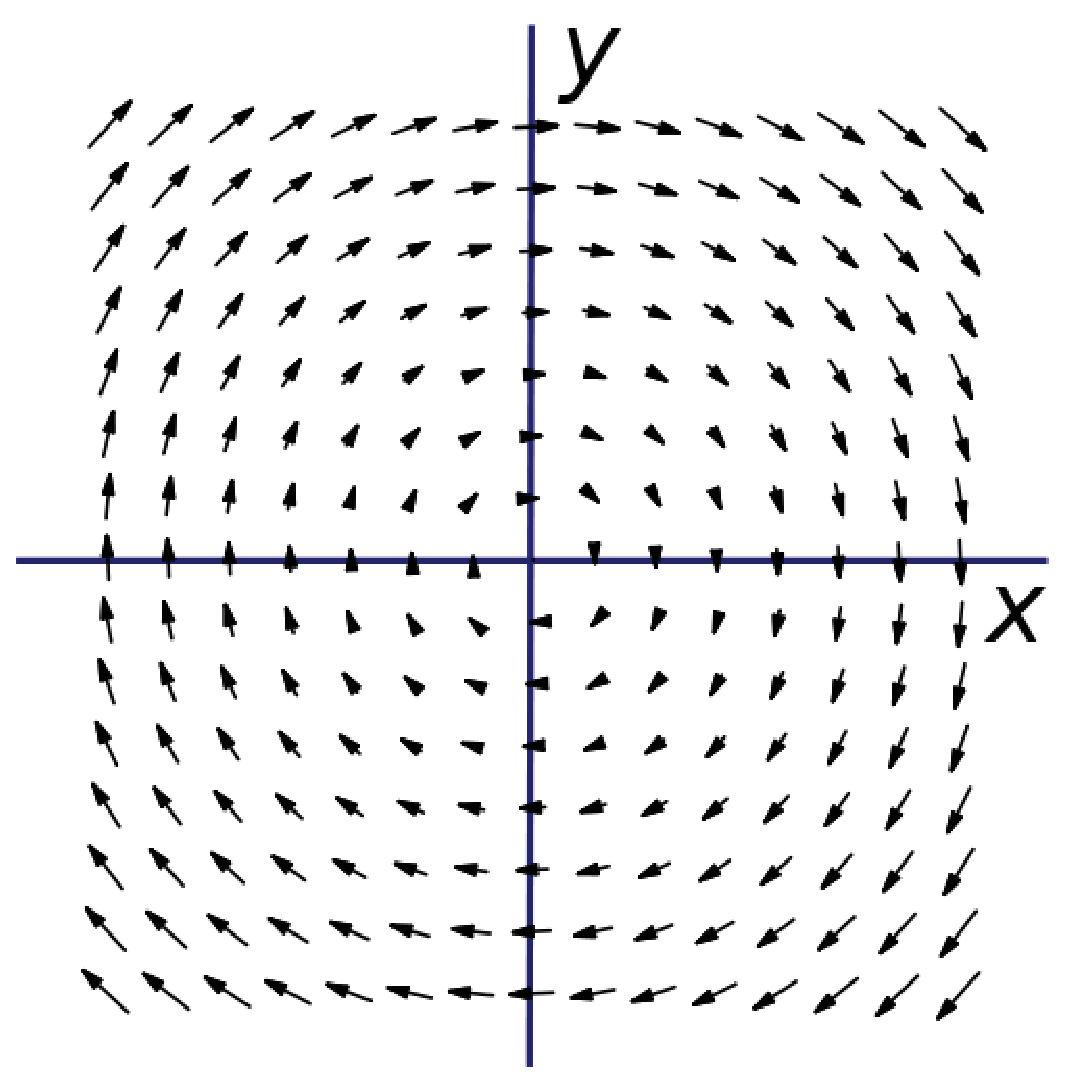
\includegraphics[width=0.25\textwidth]{Figures/curl}\\
  \end{centering}
  \caption{A simple rotation vector field in a square domain}
\end{figure}
The initial distribution of the values of the dependent variable {\scriptsize c} is a jump between the value 1 which is assigned to a square with the edge length 6, and the value 0 which is assigned to the rest of the domain.
A running solution of the Tutorial can be found in {\scriptsize C:\textbackslash BoSSS\textbackslash src\textbackslash public\textbackslash L4-application\textbackslash ScalarTransport}.
\subsubsection{Implementation of the solution procedure in BoSSS}
\paragraph{} As it was mentioned before, in BoSSS it is possible to develop a BoSSS application from a VS empty page using the available libraries provided in BoSSS project. There are also a number of BoSSS applications which are already developed, such as the present example. But because of its relative simplicity, developing this BoSSS application from a VS empty page is described in this section. This could be a start point for developing different BoSSS applications and adding more developments to the available BoSSS applications.
A running solution of the tutorial can be obtained from {\scriptsize ...\textbackslash src\textbackslash public\textbackslash L4-application\textbackslash ScalarTransport}.
\paragraph{Adding the references} A set of references corresponding to this particular BoSSS application should be added to the created VS project. In addition to the primary library file of the layers L1, L2 and L3, the library files {\scriptsize BoSSS.Foundation.grid.dll} and {\scriptsize BoSSS.Solution.Tecplot.dll} should be added.
\paragraph{The statement {\scriptsize using}} As a start point, a VS code-file with the name {\scriptsize Program.cs} is available for developing a BoSSS application. A few number of code-lines are written automatically in this code-file. The code-file is started with the statements {\scriptsize using}. This statement is used to specify that the classes which are aimed to be used, belong to a set of particular namespaces. Consequently there is no need to write the full name of a class in the code-file. For Example if the class {\scriptsize Application} is aimed to be used, taking a look at the reference manual (the file {\scriptsize BoSSS.chm}) it can be known that this class belongs to the namespace {\scriptsize Solution}. Therefore using the following code-line at the beginning of the code-file, it can be written {\scriptsize Application} as the class name instead of {\scriptsize BoSSS.Solution.Application}:
{\scriptsize \begin{verbatim}
  using BoSSS.Solution;
\end{verbatim}}
Among the default namespaces written automatically in this code-file, just the namespace {\scriptsize System} is needed to be specified by the statement {\scriptsize using}. Corresponding to the classes which should be used to develop this application, the following code-lines should be written at the beginning of the code-line {\scriptsize Program.cs}:
{\scriptsize \begin{verbatim}
  using System;
  using BoSSS.Solution;
  using BoSSS.Foundation.Grid;
  using BoSSS.Foundation;
  using BoSSS.Solution.Timestepping;
  using BoSSS.Solution.Tecplot;
  using BoSSS.Foundation.Comm;
  using BoSSS.Foundation.IO;
  using System.Diagnostics;
  using BoSSS.Foundation.Quadrature;
  using MPI.Wrappers;
  using BoSSS.Platform;
  using ilPSP.Tracing;
  using BoSSS.Solution.Utils;
  using System.IO;

\end{verbatim}}
\paragraph{The statement {\scriptsize namespace}} The code is continued using the statement {\scriptsize namespace} as the following:
{\scriptsize \begin{verbatim}
  namespace ScalarTransport {
\end{verbatim}}
This code-line covers the rest of the code-lines in this code-file, specifying that all of the classes which are defined in this code-file, belong to the namespace {\scriptsize ScalarTransport} which has the same name as the created VS project name.
\paragraph{Inharitance of the class {\scriptsize Program} from the class {\scriptsize BoSSS.Solution.Application}} Like the other developed BoSSS applications, the code-file {\scriptsize Program.cs} is assigned to define the class {\scriptsize Program} which is inherited from the large class {\scriptsize BoSSS.Solution.Application}. The code is continued as the following:
{\scriptsize \begin{verbatim}
  class Program{
\end{verbatim}}
This code-line is written automatically when the code-file {\scriptsize Program.cs} is created. As it was described in section (4.9), the inheritance should be indicated by a colon followed by the name of the class {\scriptsize BoSSS.Solution.Application}. After writing the colon sign and the first letter of the word {\scriptsize Application}, a menu appears including a list of the classes which belong to the namespaces which are specified with the statement {\scriptsize using} at the beginning of the code-file. Highlighting the word {\scriptsize Application} in the menu by the up-down arrow keys and pressing the key tab, the word {\scriptsize Application} is automatically written. Therefore the code-line converts to:
{\scriptsize \begin{verbatim}
  class Program : Application{
\end{verbatim}}
There are three ways to be informed about the members of the class {\scriptsize BoSSS.Solution.Application}:
\begin{itemize}
\item In the reference manual of BoSSS (the file {\scriptsize BoSSS.chm}) under the namespace {\scriptsize BoSSS.Solution} a brief information can be found for each member.
\item The same information as the manual reference can be found in the Metadata code-file which can be opened by right-clicking on the word {\scriptsize Application} in the code-line and selecting {\scriptsize Go To Definition} in the appeared menu.
\item In the source code-file of the class {\scriptsize BoSSS.Solution.Application} which is located in the directory {\scriptsize C:\textbackslash BoSSS\textbackslash src\textbackslash public\textbackslash L3-solution\textbackslash BoSSS.Solution}, the details of the implementations of the different members can be found.
\end{itemize}
For being informed about the members of the other classes, such ways mentioned above can be proceeded.
\paragraph{The method rmPlots}
This method is just implemented to make the program a bit more comfortable. The method deletes all .plt files in the output directory before saving the files of a new run in this directory. The implementation is straightforward and can be seen in the following.
\scriptsize \begin{verbatim}
	private static void rmPlots(){
	  var dir = new DirectoryInfo(Directory.GetCurrentDirectory());
	  Console.Write("rm");
	  foreach (var pltFile in dir.GetFiles("*.plt"))
	  {
	  Console.Write(" " + pltFile.Name);
	  pltFile.Delete();
	  }
	  Console.WriteLine(";");
	}
\end{verbatim}
\paragraph{The method {\scriptsize main}}
The code is continued by the following code-lines which are automatically written when the code-file {\scriptsize Program.cs} is created:
{\scriptsize \begin{verbatim}
  static void Main(string[] args){
  }
\end{verbatim}}
This code-line defines the method {\scriptsize main} which must be included in every C\# executable. The C\# compiler looks for this method as an entry point at the beginning of compiling. In the method {\scriptsize main} it is aimed to invoke some of the methods which belong to the class {\scriptsize Program}. Therefore the class {\scriptsize Program} should be instantiated writing the following code-line in the method {\scriptsize main}:
{\scriptsize \begin{verbatim}
   Application._Main(args, true, "BoSSS.Application,BoSSS.Solution,BoSSS.Foundation", delegate() {
   	return new Program(); });
\end{verbatim}}



\paragraph{Overriding the method {\scriptsize CreateOrLoadGrid}}
The next step is creating the numerical grid which is necessary for the numerical solution. In BoSSS the grid is generated by invoking the method {\scriptsize CreateOrLoadGrid}. This method is invoked by using the method {\scriptsize Init} of the class {\scriptsize BoSSS.Solution.Application}. By default, this method loads a grid which is created using a grid generation software and is addressed in a control file. For the present example there is no control file and it is aimed to create a grid using the grid generation capability of BoSSS. Therefore this method should be overridden by writing the following code-line:
{\scriptsize \begin{verbatim}
 protected override GridCommons CreateOrLoadGrid(){
\end{verbatim}}
For generating the two-dimensional grid in the squared domain using the BoSSS grid generator, at first two one-dimensional grids in X and Y directions should be generated by invoking the method {\scriptsize Linespace(a,b,n)} of the class {\scriptsize BoSSS.Foundation.Grid.Grid1D}. The method {\scriptsize Linespace(a,b,n)} is a static method, therefore there is no need to instantiate the class {\scriptsize BoSSS.Foundation.Grid.Grid1D} to invoke it. The first and second arguments of this method specify the minimum and maximum one-dimensional coordinate of the one-dimensional grid. The third argument specifies the number of distributed grid nodes. The generated one-dimensional grids in X and Y directions, are saved in two arrays as following:
{\scriptsize \begin{verbatim}
  double[] xnodes = Grid1D.Linspace(-7,7,20);
  double[] ynodes = Grid1D.Linspace(-7,7,20);
\end{verbatim}}
The two-dimensional grid can be generated using the class {\scriptsize Cartesian2DGrid} which has six arguments, two of them are the generated one-dimensional grids.
\paragraph{} Before describing how to use this class, the classes {\scriptsize BoSSS.Foundation.Grid.GridCommons} ,   {\scriptsize BoSSS.Foundation.Grid.GridData} and {\scriptsize BoSSS.Foundation.Context} should be briefly explained. The class {\scriptsize BoSSS.Foundation.Grid.GridCommons} is an abstract class which deals with the preliminary information about the created or loaded grids. The reason of defining this class as an abstract class is that, this class is aimed to deal with the preliminary information of every types of the numerical grids. The class {\scriptsize BoSSS.Foundation.Grid.GridData} deals with the complementary information of the created or loaded grid. These information which include the grid data structure, are based on the information in the class {\scriptsize BoSSS.Foundation.Grid.GridCommons}. Both classes are used to specify the types of two properties which are included in the class {\scriptsize BoSSS.Foundation.Context}. The class {\scriptsize BoSSS.Foundation.Context} deals with the following information:
\begin{itemize}
\item Logical information (such as the connectivity) about the created or loaded grid, which are stored in the property {\scriptsize Grid}. The type of this property is {\scriptsize BoSSS.Foundation.Grid.GridCommons}. In the other words, this property is a declaration of the class {\scriptsize BoSSS.Foundation.Grid.GridCommons}.
\item Information about the data structure of the created or loaded grid, which is stored in the property {\scriptsize GridDat}. The type of this property is {\scriptsize BoSSS.Foundation.Grid.GridData}.
\item Information about the parallel communications, which is stored in the property {\scriptsize CommmMaster}. The type of this property is {\scriptsize BoSSS.Foundation.Commm.Master}
\item IO (input/output) such as saving the grid into the BoSSS database. These information are stored in the property {\scriptsize IOMaster}. The type of this property is {\scriptsize BoSSS.Foundation.IO.Master}.
\end{itemize}
\paragraph{Creating two-dimensional grid} In the procedure of overriding the method {\scriptsize CreateOrLoadGrid}, after creating two one-dimensional grids, a two dimensional grid can be created using the class {\scriptsize BoSSS.Foundation.Grid.Catesian2DGrid} which is inherited from the class {\scriptsize BoSSS.Foundation.Grid.GridCommons}. As it was mentioned in the previous paragraph, the preliminary information of a created grid is stored in the fields and properties of the class {\scriptsize BoSSS.Foundation.Grid.GridCommons}. This class can be declared but can not be instantiated because this class is an abstract class. Therefore an object as a two-dimensional grid with the name {\scriptsize grd} and the type {\scriptsize BoSSS.Foundation.Grid.GridCommons} can be instantiated from the class {\scriptsize BoSSS.Foundation.Grid.Cartesian2DGrid}, writing the following code-line:
{\scriptsize \begin{verbatim}
  GridCommons grd = Grid2D.Cartesian2DGrid(xnodes, ynodes, CellType.Square_Linear, false, false, null);
\end{verbatim}}
As it is seen in this code-line, six initializations are taking place. Two of them use the created one-dimensional grids. The third one describes which Celltype should be used for grid generation. The forth and fifth arguments should be set{\scriptsize false} because no periodic boundary conditions are aimed to be imposed in X and Y directions. If it is needed to cut to the grid to model different shapes then a simple square domain the sixth argument should be set to {\scriptsize null}.\\
The grid is given back by returning the object grd of class GridCommons:
{\scriptsize \begin{verbatim}
  return grd;
\end{verbatim}}
This code-line performs the last task which is needed for overriding the method {\scriptsize CreateOrLoadGrid}.\\
\paragraph{Implementation of the methods with abstract modifier}
As it was mentioned before, the methods of a base class which have abstract modifier, have to be overridden in the inherited class. Correspondingly the next step in this code-file treats the implementation of the methods with abstract modifier. This can be done by right-clicking on the word {\scriptsize Application} and selecting {\scriptsize Quick Actions} (bulb symbol). There, click on the option {\scriptsize Implement Abstract Class}. Consequently the following code-lines are automatically written:
{\scriptsize \begin{verbatim}
  protected override void CreateEquationsAndSolvers(){
    throw new NotImplementedException();
  }
  protected override double RunSolverOneStep(int TimestepNo, double phystime, double dt){
    throw new NotImplementedException();
  }
  protected override void PlotCurrentState(double physTime, int timestepNo){
    throw new NotImplementedException();
  }
\end{verbatim}}
In each of these methods, the code-line {\scriptsize throw new NotImplementedException()} which should be deleted, is written just to specify that nothing is implemented in this method. Moreover, the following code-lines have to be added:
{\scriptsize \begin{verbatim}
  protected override void CreateFields(){
    throw new NotImplementedException();
  }
\end{verbatim}}
Since {\scriptsize Create Fields()} originally is a virtual method what means that this method can be implemented in a derived class but does not have to, it is not covered by the Quick Action {\scriptsize Implement Abstract Class. 
\paragraph{Creating DG field}
In the Discontinuous Galerkin method, in each cell, there is a spectrum of data for each variable, which is called DG field. This can be done in BoSSS by declaring the class {\scriptsize DGField} for every dependent mathematical variable which is involved in a particular calculation, writing the following code-line above the definition of the class CreateFields():
{\scriptsize \begin{verbatim}
  DGField c;
  VectorField<SinglePhaseField> Velocity;
  DGField mpi_rank;
\end{verbatim}}
The first two fields give the information of the physical values. The third one defines an additional parameter which is used later to plot the information which cell belongs to which process in case of calculating the solution by using mpi.
\paragraph{Overriding the method {\scriptsize CreateFields}}
In the Discontinuous Galerkin method, the DG fields are constructed on the DG basis polynomials. It can be done in BoSSS using the class {\scriptsize Basis}. By overriding the method {\scriptsize CreateFields} the following code-line should be written to instantiate the class {\scriptsize Basis} to make a DG basis for the DG field {\scriptsize c}:
{\scriptsize \begin{verbatim}
  protected override void CreateFields(){
  Basis cBasis = new Basis(this.GridData, 1);
\end{verbatim}}
The second argument in the constructor of the class {\scriptsize Basis} specifies the degree of the DG polynomial. Having the object {\scriptsize cBasis}, the class {\scriptsize Field} which was declared before , can be instantiated, as the following:
{\scriptsize \begin{verbatim}
  c = new SinglePhaseField(cBasis, "c");
\end{verbatim}}
As it can be  seen in this code-line, the object {\scriptsize cBasis} appears as first argument in the constructor of the class {\scriptsize SinglePhaseField}. The reason to declare the class {\scriptsize SinglePhaseField} outside overriding the method {\scriptsize CreateFields}, is that the variable {\scriptsize c} is aimed to be accessible for all of the methods of the class {\scriptsize Program}. Although the instantiation of the class {\scriptsize SinglePhaseField} is done by overriding the method {\scriptsize CreateFields}, for using the object {\scriptsize c} in the other methods, it is not needed to instantiate the class {\scriptsize SinglePhaseField} again. In the following the {\scriptsize DGField mpi\_rank} and the {\scriptsize VectorField Velocity} are instantiated as follows:
{\scriptsize} \begin{verbatim}
mpi_rank = new SinglePhaseField(new Basis(this.GridData, 0), "MPI_rank");
Velocity = new VectorField<SinglePhaseField>(this.GridData.SpatialDimension,
 new Basis(this.GridData, 2), "Velocity", SinglePhaseField.Factory);
\end{verbatim}
As the last task to override the method {\scriptsize CreateFields}, the following code-line should be written for adding the created field to the BoSSS database:
{\scriptsize \begin{verbatim}
  m_IOFields.Add(c);
\end{verbatim}}
\paragraph{Overriding the method {\scriptsize CreateEquationsAndSolvers}}
The next step is to introduce the scalar-transport equation of this example to BoSSS. There are two differential operators in this equation, including a temporal differential operator which is not dealt by DG, and an advective differential operator. First of all, by applying DG on the advective operator, the equation is converted to an ordinary equation including the temporal differential operator which can be solved by a temporal descritization method such as the explicit Euler method. The cells which are contained in a domain can be divided into two groups. In the first group of the cells, all of the edges of each cell are a part of the domain interior. But in the second group, each cell has at least one edge which is a part of the domain border. The cells interact together via the numerical fluxes through their edges. The formulation which is used to calculate the inner-edge fluxes is different than the formulation used to calculate the border-edge fluxes. The first task which should be done in overriding the method {\scriptsize CreateEquationsAndSolvers}, is to instantiate the class {\scriptsize BoSSS.Foundation.SpatialDifferentialOperator} writing the following code-line:
{\scriptsize \begin{verbatim}
  protected override void CreateEquationsAndSolvers() {
            SpatialOperator diffOp = new SpatialOperator(new string[] { "c" },
            BoSSS.Solution.NSECommon.VariableNames.VelocityVector(this.GridData.SpatialDimension),
            new string[] { "codom1" },
            QuadOrderFunc.Linear());
\end{verbatim}}
The class {\scriptsize BoSSS.Foundation.SpatialOperator} is used to define a spatial operator of any type. It operates on a field which is a domain variable (first argument) by using a certain parameter variable (second argument) and produces an output which is called co-domain variable (third argument). The quadrature (integration) function is chosen to be linear in this case (forth argument). Afterwards the following block should be implemented in the code. The switch following command is being used to distinguish between the case of 2 and 3 dimensional problems. For every spatial differential operator the code line which adds such an operator should be written (In this example there is only one spatial differential operator). Please note that the class {\scriptsize ScalarTransportFlux} (respectively {\scriptsize ScalarTransportFlux3D}) will be implemented later. 
{\scriptsize \begin{verbatim}
	 switch (this.GridData.SpatialDimension)
	 {
		 case 2:
			 diffOp.EquationComponents["codom1"].Add(new ScalarTransportFlux());
			 break;
		 case 3:
			 diffOp.EquationComponents["codom1"].Add(new ScalarTransportFlux3D());
			 break;
		 default:
			 throw new NotImplementedException("spatial dim. not supported");
	 }
	\end{verbatim}}
The property {\scriptsize EquationComponents} which belongs to the class {\scriptsize BoSSS.Foundation.SpatialOperator}, takes an index as a string of the name of the corresponding co-domain variable. The method {\scriptsize Add} specifies the formulation using which co-domain variable should be calculated by operating on the domain variable. In this example, the classes {\scriptsize ScalarTransportFlux} and {\scriptsize ScalarTransportFlux3D} which are explained later, are used to formulate the spatial differential operator. The instantiation of this class is done in the argument of the method {\scriptsize Add}. To finalize the procedure of introducing the spatial operators, the following code-line should be written:
{\scriptsize \begin{verbatim}
  diffOp.Commit();
\end{verbatim}}
After writing this code-line which can be done only once in the life time of the object {\scriptsize diffOp}, the spatial operator(s) can not be modified or removed. By writing the mentioned code-lines in overriding the method {\scriptsize CreateEquationsAndSolvers}, the spatial term is discretized and the equation is converted to an ordinary differential equation containing a temporal differential operator. In this example, this equation is temporally discretized using the explicit Euler method, writing the following code-line:
{\scriptsize \begin{verbatim}
  Timestepper = new RungeKutta(RungeKutta.RungeKuttaScheme.TVD3,
	  diffOp,
	  new CoordinateMapping(c), Velocity.Mapping);
\end{verbatim}}
It should be noted that like the object {\scriptsize c}, the object {\scriptsize eEuler} should also be accessible for the other methods in the class {\scriptsize Program}. Therefore it is declared before overriding the method {\scriptsize CreateEquationsAndSolvers} writing the following code-line:
{\scriptsize \begin{verbatim}
  ExplicitEuler Timestepper;
\end{verbatim}}
The class {\scriptsize ExplicitEuler} is an abstract class which can not be instantiated. Therefore the object is created with the type the class {\scriptsize ExplicitEuler} and the instantiation of the class {\scriptsize RungeKutta}.
\paragraph{Overriding the method {\scriptsize RunSolverOneStep}}
The next step is propagating in time from an initial state using the formulation which is provided by overriding the method {\scriptsize CreateEquationsAndSolvers}. This time propagation is done by overriding the method {\scriptsize RunSolverOneStep}. The number of invoking this method is equal to the number of time steps. In BoSSS it is possible to create a tracing file containing some debugging information for each time step. The following code-line provides creation of the tracing file in the BoSSS database:
{\scriptsize \begin{verbatim}
 protected override double RunSolverOneStep(int TimestepNo, double phystime, double dt) {
    using (new FuncTrace()) {
\end{verbatim}}
It should be noted that the tracing file is created only if the third argument of the method {\scriptsize run} which is invoked in the method {\scriptsize main} of the code-file {\scriptsize program.cs}, is {\scriptsize true}, even if the mentioned code-line is written in overriding the method {\scriptsize RunSolverOneStep}. The time step in BoSSS can be specified either in overriding the method {\scriptsize RunSolverOneStep} or in the control file if it does exist. If the time step is negative, it is specified in overriding the method {\scriptsize RunSolverOneStep} and vice versa. By default the time step is negative in the class {\scriptsize BoSSS.Solution.Application}. If there is a control file, which is specified in the second argument of the method {\scriptsize run} which is invoked in the method {\scriptsize main} of the code-file {\scriptsize program.cs}, the sign of the time step is converted to a positive value in the class {\scriptsize BoSSS.Solution.Application}. At first the parameter dtCFL must be introduced. It is initialized by computing a global time step size according to the Courant-Friedrich-Lax criterion:
{\scriptsize \begin{verbatim}
	double dtCFL = this.GridData.ComputeCFLTime(this.Velocity, 1.0e10);
	\end{verbatim}}
As mentioned above, if the time step is negative, it is specified by the method {\scriptsize RunSolverOneStep}. Therefore the following code-lines must be added:
{\scriptsize \begin{verbatim}
	if (dt <= 0)
	{
		dtCFL *= 1.0 / (((double)c.Basis.Degree).Pow2());
	
		base.NoOfTimesteps = 100000;
		base.EndTime = 5.0;
	}
	\end{verbatim}}
Summarizing the calculation of {\scriptsize dtCFL} both the information of the grid size and the information of the highest polynomial degree are used.
The fields {\scriptsize NoOfTimesteps} and {\scriptsize EndTime} belong the class {\scriptsize BoSSS.Solution.Application}. The value which is assigned to the field {\scriptsize NoOfTimesteps} specifies the number of time steps. The field {\scriptsize EndTime} is used to specify the time to which the propagation should be performed. The time step according to the criterion mentioned above is calculated by dividing the global time step by the highest polynomial degree of all base functions to the power of 2. To see the process of time propagation, the following code-lines should be written:
{\scriptsize \begin{verbatim}
  Console.Write("Timestp. #" + TimestepNo + " of " + base.NoOfTimesteps + " ... ");
\end{verbatim}}
To perform one time step time propagation, the following code-line should be written:
{\scriptsize \begin{verbatim}
  Timestepper.Perform(dtCFL);
\end{verbatim}}
This code-line invokes the method {\scriptsize Perform} of the class {\scriptsize ExplicitEuler}. This method takes the specified time step as an argument.
To print information of every time step and to create a Tecplot file of the result for every certain number of time steps, the following code-lines should be written:
{\scriptsize \begin{verbatim}
  Console.WriteLine("finished (dt = {0:0.###E-00}, CFL frac = {1:0.###E-00})!", dt, dt / dtCFL);
  PlotCurrentState(phystime, TimestepNo);
\end{verbatim}}
The method {\scriptsize PlotCurrentState} which is invoked, is aimed to be overridden in the class {\scriptsize Program}. The last task which should be done in overriding the method {\scriptsize RunSolverOneStep} is to return the obtained time step to be used for continuation of the time propagation. It can be done writing the following code-line:
{\scriptsize \begin{verbatim}
  return dt;
\end{verbatim}}
\paragraph{Overriding the method {\scriptsize PlotCurrentState}}
There are two codelines which should be used to overwrite the method:
{\scriptsize \begin{verbatim}
	Tecplot plt1 = new Tecplot(GridData, true, false, 0);
	plt1.PlotFields("transport_NOrec_" + timestepNo, "Scalar Transport", physTime, c, mpi_rank);
\end{verbatim}}
In the first line an object of the class Tecplot is created by getting the spatial information from the first argument of the constructor and further arguments specifying the plot appearance. In the second code-line, the method {\scriptsize PlotFields} of the class {\scriptsize BoSSS.Solution.Tecplot} is invoked to save the solution result from BoSSS database to a Tecplot file. The third argument describes the physical time at which the parameters in the forth and fifth argument should be plotted.
\paragraph{Overriding the method {\scriptsize SetInitial}}
To initialized the value of the dependent variable {\scriptsize c} and the velocity field in the domain, the virtual method {\scriptsize SetInitial} which is inherited from the class {\scriptsize BoSSS.Solution.Application}, should be overridden, because by default the initialization is done using a control file. To do the initialization, the method {\scriptsize ProjectField} of the class {\scriptsize BoSSS.Foundation.Field} should be invoked. Again, to distinguish between two different spatial dimensions, a switch block is inserted in the code:
{\scriptsize \begin{verbatim}
protected override void SetInitial(){	
  switch (GridData.SpatialDimension) {
	  case 2:
		  c.ProjectField((x, y) => ((Math.Abs(x) <= 3.0 && Math.Abs(y) <= 3.0) ? 1 : 0));
		  Velocity[0].ProjectField((_2D)((x, y) => y));
		  Velocity[1].ProjectField((_2D)((x, y) => -x));
		  break;
  
	  case 3:
		  c.ProjectField((x, y, z) => ((Math.Abs(x) <= 3.0 && Math.Abs(y) <= 3.0 && Math.Abs(z) <= 3.0) ? 1 : 0));
		  Velocity[0].ProjectField((_2D)((x, y) => 1));
		  Velocity[1].ProjectField((_2D)((x, y) => 0));
		  Velocity[2].ProjectField((_2D)((x, y) => 0));
		  break;
  
	  default:
		  throw new NotImplementedException();
  }  
\end{verbatim}}
The method {\scriptsize ProjectField} maps the field of the dependent variable {\scriptsize c} and the components of the vector {\scriptsize Velocity} to the DG field. It should be reminded that the field of each variable in DG is represented by a set of polynomials. The method {\scriptsize ProjectField} takes another method as an argument, which should be the delegate {\scriptsize ScalarFunction}. A deligate in C\# is a type that references (points) a method. Afterwards the following code lines should be written in the method {{\scriptsize SetInitial} to finish the overwriting procedure.
{\scriptsize \begin{verbatim}
     double rank = GridData.MyRank;
     int J = GridData.Cells.NoOfLocalUpdatedCells;
     for (int j = 0; j < J; j++) {
     mpi_rank.SetMeanValue(j, rank);
     }
}
\end{verbatim}}
In those code lines the information which cell belongs to which process is stored in the DGField {\scriptsize mpi\_rank}. The purpose is to get access to those values in terms of creating a plot.
\paragraph{Inheritance of the class {\scriptsize ScalarTransportFlux}}
For reasons of simplicity the following introductions are only made for 2D problems. Nevertheless in the directory {\scriptsize C:\textbackslash BoSSS\textbackslash src\textbackslash public\textbackslash L4-Applications} the definition of the TransportFlux for a 3-dimensional case can be found as well as the solution for the 2-dimensional case. \\
The formulation which is used to calculate the numerical advective fluxes through the inner-edges and border-edges is defined in the class {\scriptsize ScalarTransportFlux}. Although this class can be defined in the code-file {\scriptsize Program.cs}, to do a better code management and to prevent making a large code file, this class will be defined in another code-file but under the same namespace as the class {\scriptsize Program}. To add a code-file to a VS project the following steps should be done:
\begin{enumerate}
\item In the panel {\scriptsize Solution Explorer} under the VS solution {\scriptsize MySolution}, right-click on the VS project {\scriptsize MyProject}, and in the appeared menu, click {\scriptsize Add $\rightarrow$ New Item} to open the panel {\scriptsize Add New Item}.
\item In the panel {\scriptsize Add New Item} in the section {\scriptsize Categories} select the option {\scriptsize Code} under the subsection {\scriptsize Visual Studio Items}.
\item In the panel {\scriptsize Add New Item} in the section {\scriptsize Visual Studio Installed Templates} select the option {\scriptsize Class}.
\end{enumerate}
At the beginning of the created code-file, the following code-lines should be written to implement the statement {\scriptsize using}:
{\scriptsize \begin{verbatim}
  using System;
  using System.Collections.Generic;
  using BoSSS.Solution.Utils;
  using BoSSS.Platform.LinAlg;
  using BoSSS.Foundation;
\end{verbatim}}
The rest of the code-lines using the statement {\scriptsize using [...]}, which is automatically written, are not needed and can be deleted. The next code-line which is automatically written by the creation procedure is:
{\scriptsize \begin{verbatim}
  namespace ScalarTransport {
\end{verbatim}}
This code-line declares that this class is defined under the same namespace as the class {\scriptsize Program}. This code-line covers the rest of the code-lines in this code-file. There is a class defined in BoSSS with the name {\scriptsize BoSSS.Solution.Utils.NonLinearFlux} which provides a general context therein, different non-linear spatial differential operators can be defined. It can be done by inheritance of a new class from this class. To inherit the class {\scriptsize ScalarTransportFlux} from the class {\scriptsize BoSSS.Solution.Utils.NonLinearFlux}, the following code-lines should be written:
{\scriptsize \begin{verbatim}
  class ScalarTransportFlux : NonlinearFlux {
\end{verbatim}}
 The class {\scriptsize BoSSS.Solution.Utils.NonLinearFlux} has some abstract classes which have to be overridden. To do that, right-click on the word {\scriptsize NonLinearFlux} and in the appeared menu, select {\scriptsize Implement Abstract Class}. Then the following code-lines are written automatically:
{\scriptsize \begin{verbatim}
  protected override double BorderEdgeFlux(double time, double[] x, double[] normal, byte EdgeTag, 
	double[] Uin){
    throw new NotImplementedException();
  }
  protected override double InnerEdgeFlux(double time, double[] x, double[] normal, double[] Uin, 
	double[] Uout){
    throw new NotImplementedException();
  }
  protected override void Flux(double time, double[] x, double[] U, double[] output){
    throw new NotImplementedException();
  }
  public override IList<string> ArgumentOrdering{
    get { throw new NotImplementedException(); }
  }
\end{verbatim}}
As it was mentioned before, the code-lines implementing the statement {\scriptsize throw} should be deleted.\\
Before describing the rest of the code, the procedure of discretization of an advective term $\mathbf{\nabla}\cdot\mathbf{f}$ in DG is briefly explained. The discretization is performed by volume integration of the advective term times a test function $\phi$ which includes a set of DG polynomials, over each cell. By applying the integration by parts, the following expression can be written:
\begin{equation}
\int_\forall\left(\phi\mathbf{\nabla}\cdot\mathbf{f}\right)d\forall=\int_\forall\mathbf{\nabla}\cdot\left(\phi\mathbf{f}\right)d\forall-\int_\forall\left(\mathbf{f}\cdot\mathbf{\nabla}\phi\right)d\forall
\end{equation}
By applying the divergence theorem to the first integral in the right hand side of the equation 4, the following expression can be written:
\begin{equation}
\int_\forall\mathbf{\nabla}\cdot\left(\phi\mathbf{f}\right)d\forall=\int_{\partial\forall}\phi\left(\mathbf{f}\cdot\mathbf{n}\right)dA
\end{equation}
Calculation of the vector $\mathbf{f}$ of the second term in the right hand side of the equation 4 is done by overriding the method {\scriptsize Flux}. Calculation of the the flux $\mathbf{f}\cdot\mathbf{n}$ in the right hand side of the equation 5 is done by overriding the method {\scriptsize BorderEdgeFlux} for the border edges and the method {\scriptsize InnerEdgeFlux} for the inner edges.\\
The following code-line defines the method {\scriptsize Inflow} which has {\scriptsize time} as an argument and returns a value. This method is needed for overriding the method {\scriptsize BorderEdgeFlux}.
{\scriptsize \begin{verbatim}
  double Inflow(double time) {
    return 0.0;
  }
\end{verbatim}}
The prescribed vector field {\scriptsize u} is defined as a method of the type {\scriptsize Vector2D}, writing the following code-lines:
{\scriptsize \begin{verbatim}
  Vector2D FlowField(double[] x, double[] Uin, double[] Uot){
  Vector2D u;
  u.x = 0.5 * (Uin[1] + Uot[1]);
  u.y = 0.5 * (Uin[2] + Uot[2]);
  return u;
  }
\end{verbatim}}
Please note that all variables (e. g. concentration, velocity, density, etc.) are stored in the vector \verb|Uin| and \verb|Uot|. That's way in this case the velocity components that are used for calculating \verb|u.x| and \verb|u.y| are stored in the second and third entry of the array. The first entry of the array is the unknown concentration \verb|c|. The type {\scriptsize Vector2D} provides some features of the two-dimensional vector analysis. For example the suffixes {\scriptsize .x} and {\scriptsize .y} declare the x and y coordinates of the vector {\scriptsize u} which has the type {\scriptsize Vector2D}.\\
The formulation which is used to calculate the flux $c\mathbf{u}\cdot\mathbf{n}$ through the border edges, is implemented by writing the following code-lines:
{\scriptsize \begin{verbatim}
protected override double BorderEdgeFlux(double time, double[] x, double[] normal, byte EdgeTag, 
  double[] Uin, int jEdge){
  Vector2D n; 
  n.x = normal[0]; 
  n.y = normal[1];
  var vel = FlowField(x, Uin, Uin);
  if (n * vel >= 0)
	  return (vel * Uin[0]) * n;
  else
	  return (vel * Inflow(time)) * n;
  }
\end{verbatim}}
The border edge normal vector which points outward the cell, is represented by {\scriptsize n} which has the type {\scriptsize Vector2D}. An upwind scheme is used to calculate the flux. According to this scheme, if the prescribed vector {\scriptsize u} on the border edge has the same direction as the normal vector {\scriptsize n}, the flux is the production of the vector {\scriptsize u} and the dependent variable {\scriptsize c}, times the unit normal {\scriptsize n}. Otherwise, the flux is the production of the vector {\scriptsize u} and the value which is returned by the method {\scriptsize Inflow}, times the unit normal {\scriptsize n}. The dependent variable {\scriptsize c} on the border edge is always represented by {\scriptsize Uin}.\\
The formulation which is used to calculate the flux $c\mathbf{u}\cdot\mathbf{n}$ through the inner edges, is implemented by writing the following code-lines:
{\scriptsize \begin{verbatim}
  protected override double InnerEdgeFlux(double time, double[] x, double[] normal, double[] Uin, 
    double[] Uout, int jEdge) {
    Vector2D n;
    n.x = normal[0];
    n.y = normal[1];
    if (FlowField(x, Uin, Uout) * n > 0)
      return (FlowField(x, Uin, Uout) * Uin[0]) * n;
    else
      return (FlowField(x, Uin, Uout) * Uout[0]) * n;
  }
\end{verbatim}}
It should be pointed that in DG, there is a discontinuity of the dependent variables on each inner edge. It means that there are two values for the dependent variable on an inner edge, one of them belongs to one cell and the other one belongs the other cell. Both are connected by sharing an inner edge. These two values are represented by {\scriptsize Uin} and {\scriptsize Uout}. The array {\scriptsize Uin} is assigned to the cell which the normal vector points outward it, and the array {\scriptsize Uout} belongs the cell which the unit normal point toward it. In BoSSS on each inner edge a single normal vector {\scriptsize n} is defined. In the calculation of the flux through the inner edges, the same upwinding scheme is used as for the border edges.\\
 To calculate the vector $\mathbf{f}$ of the second term in the right hand side of the equation 4, the following code-lines are written:
{\scriptsize \begin{verbatim}
  protected override void Flux(double time, double[] x, double[] U, double[] output) {
    Vector2D o;
    o = FlowField(x, U, U) * U[0];
    output[0] = o.x;
    output[1] = o.y;
  }
\end{verbatim}}
The array {\scriptsize U} represents the value of the dependent variable {\scriptsize c} on all of the edges, including the inner and border edges.
{\scriptsize \begin{verbatim}
public override IList<string> ArgumentOrdering {
   get { return new string[] { "c" }; }
   }
  
public override IList<string> ParameterOrdering {
   get { return BoSSS.Solution.NSECommon.VariableNames.VelocityVector(2);
   }
}
}
}
\end{verbatim}}
The object {\scriptsize ArgumentOrdering} is defined as an abstract class and therefore it must be overridden by using the arguments in the order wanted. The second object stores the order of all parameters and is implemented only virtual. Caused by that it only has to be overridden if parameters exist like in the current case.


\subsection{IP discretization of a Poisson equation}

The next natural step is the discretization of a second order PDE using the Symmetric Interior Penalty Galerkin (SIPG) approach. An exemplary implementation can be found in the project \verb|L4-application/ipPoisson|. Here, we only briefly summarize some frequently asked questions.

\begin{description}
	\item[What are the domain and codomain variables?] See fdy annual fdy report 2009 by Florian Kummer
	\item[How big is the created operator matrix \textit{LaplaceMtx} and the Affine Offset \textit{LaplaceAffine}?] The number of columns of the matrix is the same as the amount of global DOF. The number of rows is the same as the number of equations (number of codomains) times the number of basis polynomials, which is the same as the number of local DOF in each cell times the number of cells. This is not true if p enrichment is used, which is not the case. The affine offset is a double array with as much entries as there a global DOF.
	\item[What is an interior penalty flux?] See (Shahbazi, K., An explicit expression for the penalty parameter of the interior penalty method, 2004) and (Klein, A simple based discontinuous Galerkin solver for steady incompressible flows, 2012)
	\item[Why does the third order SinglePhaseField T have 10 columns and 400 rows for a 20x20 grid?] The polynomial degree is 3, which leads to 10 DOF per cell and 400 cells. This means 4000 global DOF.
	\item[Are Dirichlet boundary conditions only satisfied in a weak form?]See \verb|.\fdy_publications\notes\2014\FluxesAndBoundaryConditions|
\end{description}



%==================== Literatur =====================================
% Bibliography
% -------------
%\bibliography{BibDaten}
%==================== Anhang ========================================
%\appendix

\clearemptydoublepage

\end{document} 